\section{With load}
\subsection{Full-state}
The full-state feedback controller seems to get into trouble when adding a weight of 0.1. Figure~\ref{fig: full state unadjusted , not strong enough } displays the path taken by the quad copter with load. The weight of 0.1 pushes the quad copter down on the z-axis, and the controller does not compensate enough. If the weight corresponding to z is increased from $10^2$ to $10^4$ the controller does however compensate enough.(see Figure~\ref{fig: full state , strong enough }, the average time is  2.929 s)
\begin{figure}[H]
	\centering
	\begin{subfigure}[b]{0.3\textwidth}
		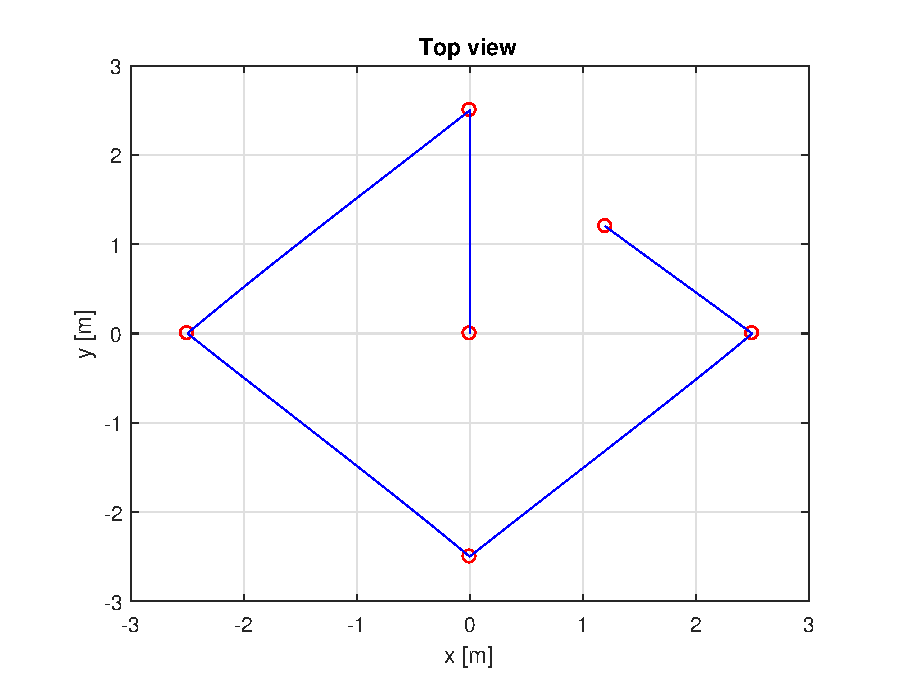
\includegraphics[width=\textwidth]{./LQR_load/fullState/noadjustment_fig1.eps}
		\caption{top view}
	\end{subfigure}
	\begin{subfigure}[b]{0.3\textwidth}
		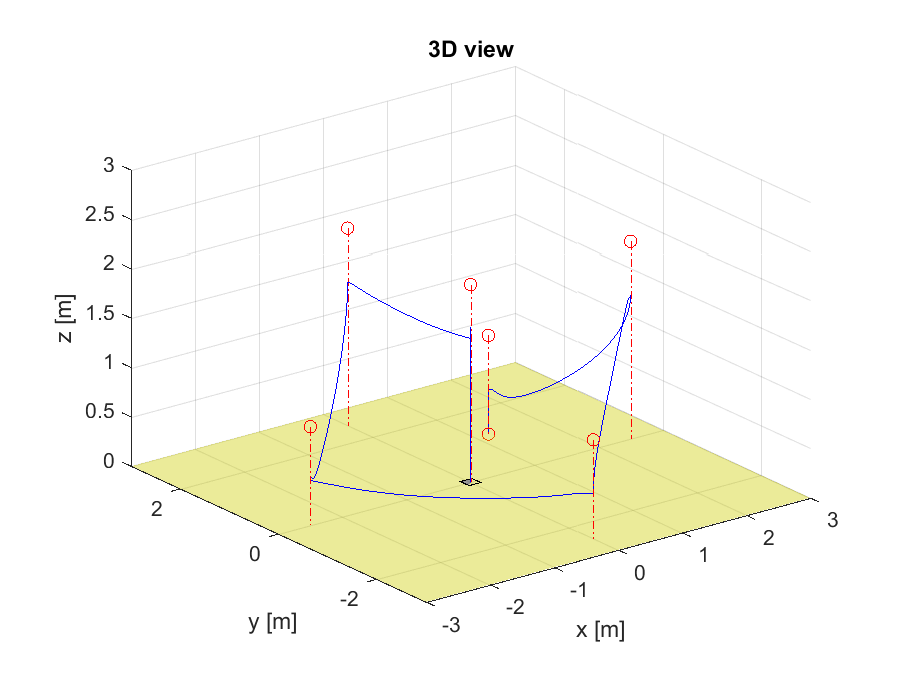
\includegraphics[width=\textwidth]{./LQR_load/fullState/noadjustment_fig2.eps}
		\caption{3D view}
		\label{fig: full state unadjusted , not strong enough }
	\end{subfigure}
	\begin{subfigure}[b]{0.3\textwidth}
		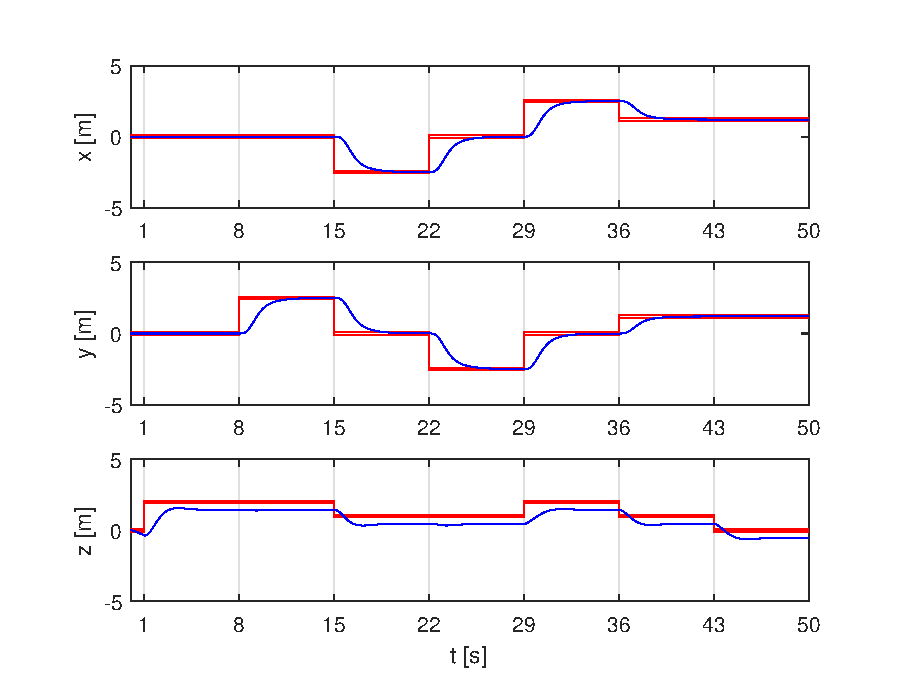
\includegraphics[width=\textwidth]{./LQR_load/fullState/noadjustment_fig3.eps}
		\caption{individual axis}
	\end{subfigure}
	\begin{subfigure}[b]{0.3\textwidth}
		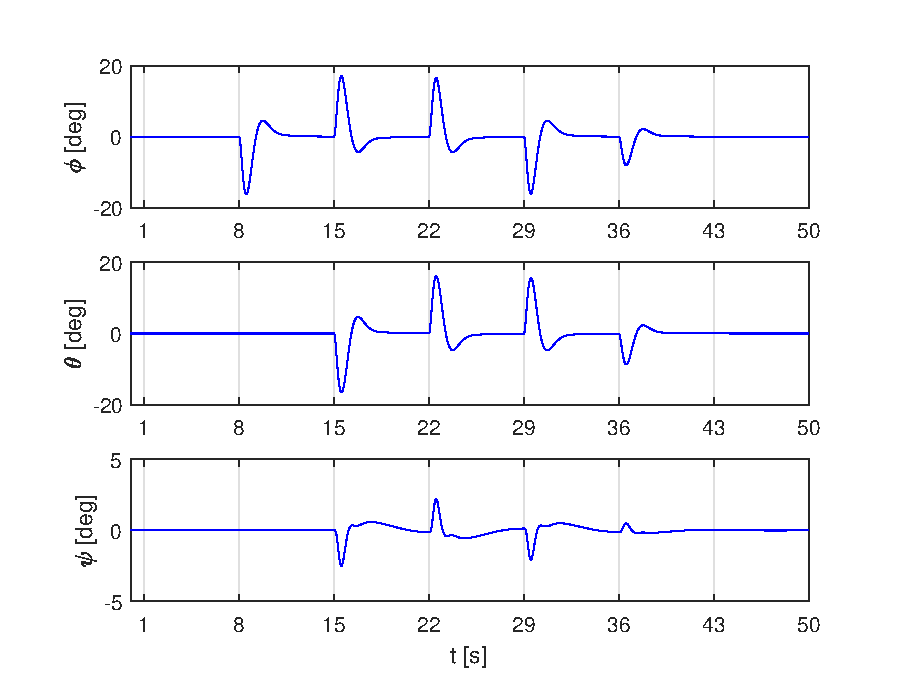
\includegraphics[width=\textwidth]{./LQR_load/fullState/noadjustment_fig4.eps}
		\caption{angles}
	\end{subfigure}
	\begin{subfigure}[b]{0.3\textwidth}
		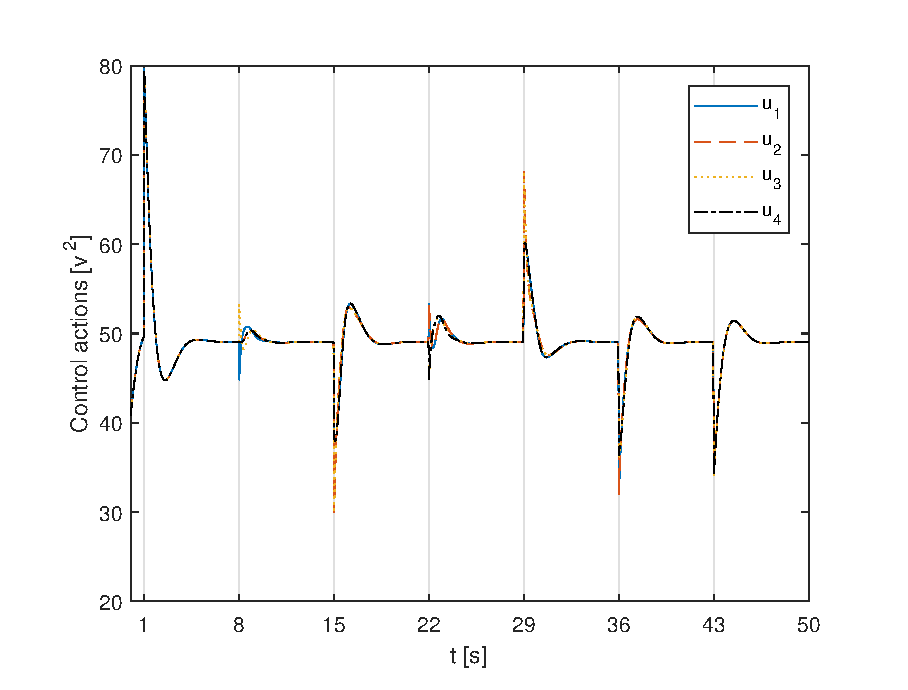
\includegraphics[width=\textwidth]{./LQR_load/fullState/noadjustment_fig5.eps}
		\caption{control actions}
	\end{subfigure}
	\caption{full state with 0.1 load, no adjustments to the weight matrices from the previous section }\label{fig:full state with load unadjusted}
\end{figure}

\begin{figure}[H]
	\centering
	\begin{subfigure}[b]{0.3\textwidth}
		\includegraphics[width=\textwidth]{./LQR_load/fullState/fig1.eps}
		\caption{top view}
	\end{subfigure}
	\begin{subfigure}[b]{0.3\textwidth}
		\includegraphics[width=\textwidth]{./LQR_load/fullState/fig2.eps}
		\caption{3D view}
		\label{fig: full state , strong enough }
	\end{subfigure}
	\begin{subfigure}[b]{0.3\textwidth}
		\includegraphics[width=\textwidth]{./LQR_load/fullState/fig3.eps}
		\caption{individual axis}
	\end{subfigure}
	\begin{subfigure}[b]{0.3\textwidth}
		\includegraphics[width=\textwidth]{./LQR_load/fullState/fig4.eps}
		\caption{angles}
	\end{subfigure}
	\begin{subfigure}[b]{0.3\textwidth}
		\includegraphics[width=\textwidth]{./LQR_load/fullState/fig5.eps}
		\caption{control actions}
	\end{subfigure}
	\caption{full state with 0.1 load with adjustments to the weight matrices from the previous section, average time is 2.929 s }\label{fig:full state with load}
\end{figure}

\subsection{Integrator}
The Integrator seems to work just fine with the load. Its a bit slower as it takes about 3.4s now to complete the track. But contrary to the full-state feedback it does finish the track unadjusted. (results displayed in Figure~\ref{fig:Integrator with load}).

\begin{figure}[H]
	\centering
	\begin{subfigure}[b]{0.3\textwidth}
		\includegraphics[width=\textwidth]{./LQR_load/Integrator/fig1.eps}
		\caption{top view}
	\end{subfigure}
	\begin{subfigure}[b]{0.3\textwidth}
		\includegraphics[width=\textwidth]{./LQR_load/Integrator/fig2.eps}
		\caption{3D view}
	\end{subfigure}
	\begin{subfigure}[b]{0.3\textwidth}
		\includegraphics[width=\textwidth]{./LQR_load/Integrator/fig3.eps}
		\caption{individual axis}
	\end{subfigure}
	\begin{subfigure}[b]{0.3\textwidth}
		\includegraphics[width=\textwidth]{./LQR_load/Integrator/fig4.eps}
		\caption{angles}
	\end{subfigure}
	\begin{subfigure}[b]{0.3\textwidth}
		\includegraphics[width=\textwidth]{./LQR_load/Integrator/fig5.eps}
		\caption{actions}
	\end{subfigure}
	\caption{integrator with 0.1 load, average of 3.393 s}\label{fig:Integrator with load}
\end{figure}

\subsection{Comparison}
The full-state feedback controller can only steer on the current situation. So when the x,y and z coordinates are different from the track it will compensate for this at a constant rate. It doesn't matter how long the copter is off the track it will keep compensating at this constant rate. 

The Integrator on the other hand will integrate the difference and so at first it will only compensate slightly but the longer the copter is off track the harder it will compensate. This is also the reason why the integrator over compensates, and an additional weight must be set to the speeds $v_x$,$v_y$ and $v_z$.

The integrator is a discrete integrator with equal distance points, and equal weights to each value. If the Integrator has 20 high values then 3 low values will not significantly change the integration value. But 10 low values will significantly change the integration value.